\documentclass[%
12pt,
twoside,
reprint,
amsmath,amssymb,
aps,
]{article}

%PDF Searchable copyable, fix symbols
\usepackage{cmap}
\usepackage[T1]{fontenc}

%Page numbers
\pagestyle{plain}

%Math Symbols
\usepackage{amsmath}
\usepackage{gensymb}
\usepackage{xfrac} %different fractions
\usepackage{bm} %bold

%Images
\usepackage{graphicx}
\usepackage{subfig}
\usepackage{caption}
\usepackage[export]{adjustbox} %scaling

%Tables
\usepackage{float,tabularx} %alternative table layout
\usepackage{dcolumn} %aligning decimals
\usepackage{makecell} %used for multi-line cells
\newcolumntype{Y}{>{\raggedleft\arraybackslash}X} %used with tabularx for sizing columns
\newcolumntype{Z}{>{\centering\arraybackslash}X}  %used with tabularx for sizing columns
\newcolumntype{?}{!{\vrule width 2pt}} %bold vertical line in table
\setlength{\extrarowheight}{5pt} %spacing between rows

%Text/paragraph formatting
\usepackage{indentfirst}
\usepackage{setspace} 
\usepackage{listings} %for displaying code
\usepackage{color, soul} %for highlighting text

%Shapes/geometries
\usepackage{tikz}
\usetikzlibrary{calc, shapes}

%Page formatting
\usepackage[margin=1in]{geometry}

%Section title formating - spacing
\usepackage{titlesec}
\titlespacing*{\section}{0pt}{0.5\baselineskip}{0.5\baselineskip}
\titlespacing*{\subsection}{0pt}{0.5\baselineskip}{0.5\baselineskip}
\setlength{\belowcaptionskip}{-10pt}

%Table of Contents
\usepackage{hyperref}
\hypersetup{ %Hyplink to location
	colorlinks,
	citecolor=black,
	filecolor=black,
	linkcolor=black,
	urlcolor=black
}
%\usepackage[indentunnumbered]{unnumberedtotoc}

%Line Numbers
\usepackage{lineno}
%\linenumbers

\begin{document}
	\thispagestyle{empty}
	\begin{center}
		\begin{minipage}{0.75\linewidth}
			\centering
			{\uppercase{\Large Manual For Using GEANT4 with the Drexel Bubble Chamber \par}}
			\vspace{3cm}
		\end{minipage}
	\end{center}
	
	\tableofcontents
	
	\raggedbottom
	\pagebreak
	
	\section{Introduction}
	\par As part of my senior thesis for graduating in June 2019, I adapted the GEANT4 software to the Drexel Bubble Chamber, wrote some analysis code, and wrote some bash scripts for automating many functions. I spent many months painfully learning and figuring out how to work with GEANT, so hopefully this manual will save you many of the troubles that I faced. 
	\par Within the manual, I will show how to get started with GEANT and the PICO code, how to run it, go through my scripts and code, and explain some of the common issues that I ran in to. It's not necessary to follow everything step by step, so skip around to what you actually need. In the spirit of helping future people who might work with this code, you should update this manual with any changes, challenges you faced, etc. to help facilitate the transition of knowledge.\\
	
	\noindent If you do run in to any issues that you can't seem to solve, feel free to contact me at: {\href{mailto:salvatorezerbo37@gmail.com}{\color{blue}\underline{salvatorezerbo37@gmail.com}}}.
	I'll try my best to respond in a timely matter with useful advice but don't get your hopes up.
	
	\section{Setup}
	\par Hopefully you have access to a linux machine, since operating GEANT on windows is a nightmare, and my scripts/code were all written on a linux machine. If you don't have one, it's never too late to set up a linux dual boot on your laptop. It's fairly quick, easy, and is extremely useful to have when you need it. I have no idea how anything works on mac, so you're on your own there for installation and adapting the scripts as necessary. For reference, below is a list of versions of everything that I used. These versions might not be necessary, but if you run in to issues, try to obtain something similar.
	\begin{table}[!h]
		\centering
		\footnotesize
		\begin{tabular}{l|l}
			\textbf{Software} & \textbf{Version} \\ \hline
			Linux & Mint 18.3 (Sylvia)\\
			Bash & 4.3.48(1)-release \\
			GEANT4 & 10.3 (From SVN) \\
			Python & 3.5.2 \\
			\ \ --Pandas & 0.24.1 \\
			\ \ --Numpy & 1.16.2 \\
			\ \ --Matplotlib & 3.0.3 \\
			\ \ --astroML & 0.4 \\
			\ \ --astropy & 3.1.2 \\
		\end{tabular}
	\end{table}

	\subsection{Accounts}
	\par In order to access the SVN that contains the PICO GEANT code, you will need to have a Snolab account. I had already obtained my Snolab account from my brief visit to Snolab, so I cannot say too much on this. Professor Neilson should be able to guide you to getting an account.
	\par I don't believe you need to obtain Fermilab accounts for the purpose of the GEANT simulations, but it might be useful to also get it out of the way during this stage if you think you'll need it for other purposes. Docdb 903 has a guide for obtaining a Fermilab account.
%	
	\subsection{Obtaining the GEANT Code}
	\par The SVN repository already contains a version of GEANT4 along with the code for the DBC and other chambers. To obtain the code, follow the steps on slide 3 of Docdb 3482. After cloning the svn and following the steps from the slides, your file structure should like the one seen below in Figure 1. For simulations with the DBC, you will primarily interact with code within the pico-svn/DBC-from-40/ file structure.
	
	\begin{figure}[!b]
		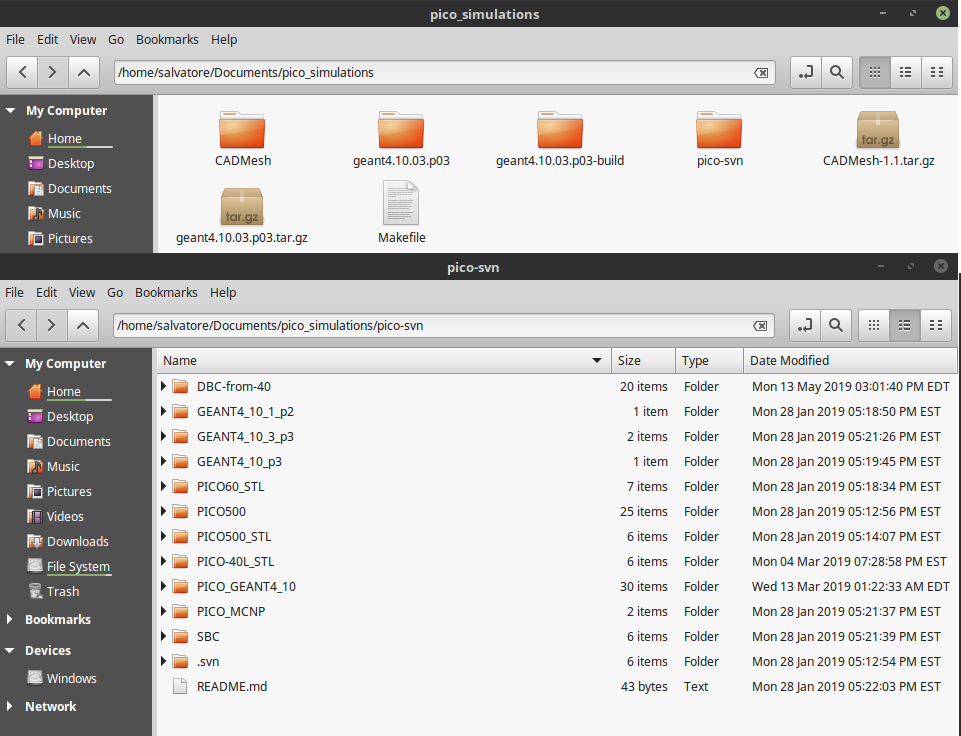
\includegraphics[scale = 0.65]{Images/svn_file_structure_test.png}
		\caption{\label{tab:table-name}}
	\end{figure}
	
	\section{Running GEANT}
	\par In this section, I'll go over how to run the simulations, make changes to the DBC construction, set up different sources with macro files, and explain the bash scripts I wrote to automate much of the process. Before jumping in to the DBC code, it may be helpful to become familiar with GEANT4 through the examples given. These are found under the file structure geant4.10.03.p03/share/Geant4-10.3.3/examples.
	
	\begin{figure}[!t]
		\centering
		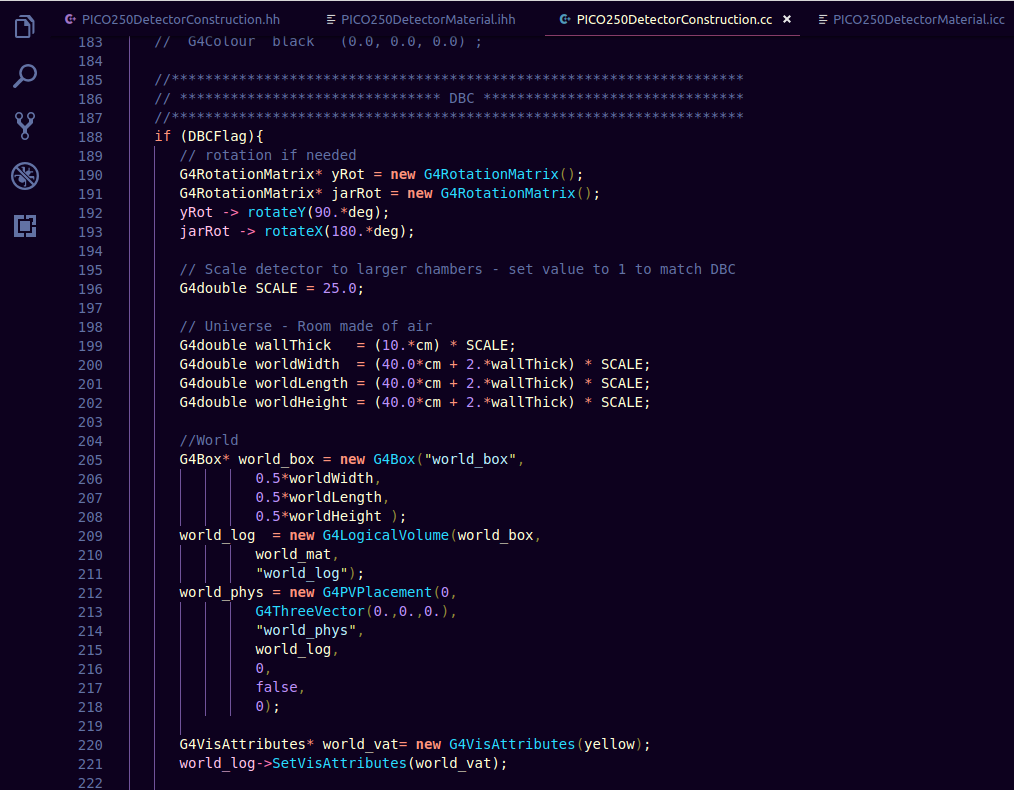
\includegraphics[scale = 0.55]{Images/detector_construction_cc_test.png}
		\caption{\label{tab:table-name}}
	\end{figure}
	
	\subsection{Adding New Components to the Chamber}
	\par The last version of the DBC that I constructed within the simulations is fairly simple, so I'm sure you'll want to know how to add more to it for more accurate simulations. Again for everything related to the DBC, all file paths I list will have an implied pico-svn/DBC-from-40 in front of them. The primary files that need to be edited to add additional components are as follows: \\
	
	\noindent include/PICO250DetectorConstruction.hh \\
	include/PICO250DetectorMaterial.ihh \\
	src/PICO250DetectorConstruction.cc \\
	src/PICO250DetectorMaterial.icc
	
	\subsubsection{PICO250DetectorConstruction.cc}
	
	\par The first step is to create the component within the PICO250DetectorConstruction.cc file. You should open the file and scroll down until you see a large commented out header saying DBC, as seen in Figure 2. All code written should be contained within the if (DBCFlag) statement. Hopefully you have some idea as to what generic shape you would like to use to model the component. I primarily used the G4Tubs, which is a cylinder, and the G4Polycone, which is a radially defined object used for the C$_{3}$F$_{8}$ and its container.

	\noindent First, you should define the dimensions of the object you are trying to create. As an example, I'll go through the code of constructing a generic cylinder, abbreviated GC in the code. The first group of code might look something like: \\
	
	\noindent G4double GCRadius = 5. * cm; \textbackslash\textbackslash GEANT4 has its own units defined conveniently \\
	G4double GCHeight = 5. * cm;
	
	\noindent G4double GCPosZ   = 10. * cm; \textbackslash\textbackslash You can define other position coordinates, but I pretty
	\indent \indent \indent \indent \indent \indent \indent \indent \indent \ \ \ \textbackslash\textbackslash much only cared about the z-axis. \\
	
	\noindent Next, you'll want to actually define the object, set its dimensions, give it a logical volume, and give it a physical volume.
	
	\begin{table}[!h]
		\begin{tabular}{ll}
			G4Tubs* GC = & \textbackslash\textbackslash Set the cylinder's dimensions \\
			\hspace{5mm} new G4Tubs("GC", & \textbackslash\textbackslash Name for referencing\\
			\hspace{10mm} 0.*cm, & \textbackslash\textbackslash Inner radius \\ 
			\hspace{10mm} GCRadius, & \textbackslash\textbackslash Outer radius \\
			\hspace{10mm} 0.5*GCHeight, & \textbackslash\textbackslash Height extends in -z and +z \\
			\hspace{10mm} 0.*deg, & \textbackslash\textbackslash Starting angle \\
			\hspace{10mm} 360.*deg); & \textbackslash\textbackslash Ending angle \\
			GC\_log = & \textbackslash\textbackslash Define the logical volume \\
			\hspace{5mm} new G4LogicalVolume(GC, & \textbackslash\textbackslash Attach to the object \\
			\hspace{10mm} GC\_mat, & \textbackslash\textbackslash Material as defined in DetectorMaterial files \\
			\hspace{10mm} "GC\_log"); & \textbackslash\textbackslash Name for referencing\\
			GC\_phys = & \textbackslash\textbackslash Define the physical volume \\
			\hspace{5mm} new G4PVPlacement(0, & \textbackslash\textbackslash Rotation matrix to rotate object \\
			\hspace{10mm} G4ThreeVector(0.,0.,GCPosZ), & \textbackslash\textbackslash Position \\
			\hspace{10mm} "GC\_phys", & \textbackslash\textbackslash Name for referencing \\
			\hspace{10mm} GC\_log, & \textbackslash\textbackslash Attach to logical volume \\
			\hspace{10mm} world\_phys, & \textbackslash\textbackslash Mother physical volume to position relative to \\
			\hspace{10mm} false, & \textbackslash\textbackslash Currently unused, always false \\
			\hspace{10mm} 0); & \textbackslash\textbackslash Overlap check \\
		\end{tabular}
	\end{table}

	\noindent The final step in this file is to add the visibility attributes. Here, the color is set and the visibility is set to true
	
	\begin{table}[!h]
		\begin{tabular}{ll}
			G4VisAttributes* GC\_vat = new G4VisAttributes(magenta); & \textbackslash\textbackslash Set color \\	
			GC\_vat->SetVisibility(true); & \textbackslash\textbackslash Set visibility true \\
			GC\_log->SetVisAttributes(GC\_vat); & \textbackslash\textbackslash Attach visibility attributes \\
		\end{tabular}
	\end{table}

	\subsubsection{Other Files}
	\par These next steps are all extremely simple compared to the previous file, so I will combine them all together here. In these files, you can place the new lines of code pretty much anywhere, though make sure you can find them again. Next navigate to the include/PICO250DetectorConstruction.hh file. Here, you'll want to add 2 new lines of code to define the logical and physical volumes set in the previous step. This will look like: \\
	
 	\noindent G4LogicalVolume* GC\_log; \\
	G4PhysicalVolume* GC\_phys; \\
	
	\noindent And that's all for that file! Next navigate to include/PICO250DetectorMaterial.ihh. Here, add 1 line: \\
	
	\noindent G4Material* GC\_mat; \\
	
	\noindent Finally, go to src/PICO250DetectorMaterial.icc. If the material you want to use is already defined, then this step is as simple as the others. Just add the following line to the code: \\
	
	\noindent GC\_mat = metalAl; \textbackslash\textbackslash I set this to aluminum, but it can be anything \\
	
	\noindent If the material you want to use is not already defined, then you should follow the example below and add it a bit further up in the same file. Here I show how to create a material for Beryllium Oxide: \\
	
	\noindent G4Material* BeO = new G4Material(name = "BeO", density = 3.02*g/cm3, \\
	\indent \indent \indent \indent \indent \indent \indent \indent \indent \indent \indent ncomponents = 2); \\
	BeO->AddElement(Be, 1); \\
	BeO->AddElement(O, 1); \\
	
	\noindent Fairly simple. The ncomponents defines how many different elements there are in your composition. Each element is then added, and you can specify how many atoms of that element there are. With this, you're all done constructing, and you are now ready to compile the code to run.
	
	\subsection{Bash Scripts For Automation}
	\par There are three bash scripts that I wrote for aiding in compiling the code and a few other useful features. These files are all contained withing the build/ directory, and you should make sure each file has proper permissions. If it does not, you can change them with the command "chmod 700 file.sh". 
	
	\par The first file we'll look at is the compile.sh file. This is the primary file that I used for compiling, running macros, storing data, etc. In fact, the remaining two bash scripts rely heavily on this script. At the top of the file, you should see two commented out lines. These lines set the source directories for GEANT and CADMesh. You should either uncomment these lines, or set the paths in your .bashrc file. If you do not set them, you will run into errors compiling. The two lines beginning with "cmake" should be updated to reflect the full path to GEANT and the full path to the build directory. Next, I'll describe the parameters for the script:
	\begin{table}[!h]
		\begin{tabular}{ll}
			guiType & \makecell[l]{- "pico", "gun", "nomake" \\
			\indent Compile for certain macro commands or don't make, see next section.}\\
			runScript & \makecell[l]{- "piconovis", "gpsnovis", "norun" \\
			\indent Choose to run macro from console, no visualization. If empty, opens gui.}\\ 
			particleScript & \makecell[l]{- "neutron", "gamma", "cm" (gps only) \\
			\indent Choose macro file to run, should update with you're own if necessary} \\
			moveOutput & \makecell[l]{- "move" \\
			\indent Moves the output of the simulations to archive folder with date if set.} \\
			fileName & \makecell[l]{- Anything \\
			\indent If moveOutput set, adds descriptor to filename such as: gamma\_\$fileName.root}
		\end{tabular}
	\end{table}

	\par The next file to look at is run\_multiple.sh. This file is used to automate the running of n simulations. You should already have compiled whatever changes that you may have made to the source code, and changes to the macro files you would like to use should also be made. This script draws two random numbers to set the seeds in the macro file and runs as many times as you would like. The seeds used are output to a file to be used again if desired. There are a few changes you can make here: \\
	
	\noindent 1. line=`grep "/random/setSeeds" neutron.mac` \\
	2. sed -i "s|\$line|/random/setSeeds \$seedOne \$seedTwo|g" neutron.mac \\
	3. ./compile.sh nomake piconovis neutron move "25x\_\$i" \\
	
	\noindent In the first and second lines, you should replace neutron.mac with the macro file that you would like to run. In the third line, you should make sure to compile with either pico or gun as appropriate and change the name of the files to reflect what you would like them to be called. \\
	
	\par The final bash script I wrote is run\_multiple\_from\_file.sh, which is an extension of the previous file to run the simulations using seeds already used previously. This will allow you to rerun simulations to reproduce results, restart simulations if they have to be interrupted for some reason, and set your own custom seeds. The same three lines as the previous file can still be altered. In addition, at the end of the while loop, you should replace "done < neutron\_seeds\_18mm.txt" with the file containing your seeds that you would like to run.
	
	\subsection{Setting Up Macro Files}

	\par Macro files, which are files ending in the ".mac" extension, are used to define the type of source and its properties such as location, isotope, strength, position, size, etc. Several other simulation parameters such as the number of events, seeds, output verbosity, etc are also set here. There are two types of sets of commands that I used: "gun" and "pico". These commands can only be used when compiled with the corresponding variable set, as described in the previous section. The pico commands should be fine for most of the applications you may want. The gps command set is useful for defining a custom emission spectrum of the source and setting a custom angular distribution for the direction that the particles are emitted.
	
	\par Here, I'll run through the basics of the neutron and gamma.mac files that I used for simulating a $^{207}$Bi gamma source with a $^9$Be target. I'll break down the macro files in groupings of parameters with the neutron file on the left and the gamma file on the right. The first group is the verbosities. These parameters control how much output there is to the console or to the GUI; however, they do not control the actual data that is output to the files. These commands are useful for checking event by event results and can be piped to an output file for storing the output.
	
	\begin{figure}[!h]
		\centering
		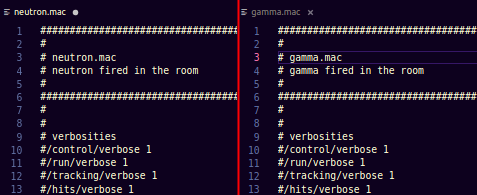
\includegraphics[scale = 1]{Images/verbosities.png}
		\caption{\label{tab:table-name}}
	\end{figure}

	\noindent The next grouping is the draw parameters. These control the colors, which lines are drawn, and which events are saved. The saveNeutron flag here will only save nuclear recoils in the target volume. The saveGamma flag will save all recoils with the target volume, including nuclear recoils. It is important to only set one or the other, otherwise you will double count hits.

	\begin{figure}[!h]
	\centering
	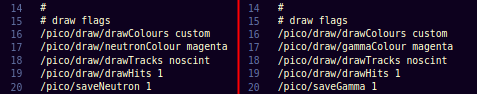
\includegraphics[scale = 1]{Images/draw.png}
	\caption{\label{tab:table-name}}
	\end{figure}
	\pagebreak
	\noindent The next two flags determine the output of the results. The primary flag here is the savePMT flag, which will output to a file specified further down. This file is what I used with my Python code to perform the analysis of the results. I'm not sure if the saveHits flag affects the results, so I've left it set to true. I also am not sure why the results of the simulation are output to a PMT file instead of the hits file, considering there is no PMT for the DBC, but that seems to be how it is.

	\begin{figure}[!h]
		\centering
		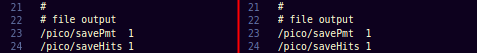
\includegraphics[scale = 1]{Images/file.png}
		\caption{\label{tab:table-name}}
	\end{figure}

	\noindent The flags here set which detector is currently being used. This is useful if you end up doing simulations on other detectors for some reason. If you recall back to the PICO250DetectorConstruction.cc file with the DBCFlag variable, there are certain properties and physics attached to each detector.

	\begin{figure}[!h]
		\centering
		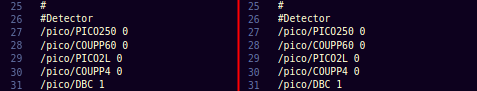
\includegraphics[scale = 1]{Images/detectors.png}
		\caption{\label{tab:table-name}}
	\end{figure}

	\noindent This line is fairly self-explanatory. I'm not sure how relevant it is for the DBC, so I've left it set to false.
	
	\begin{figure}[!h]
		\centering
		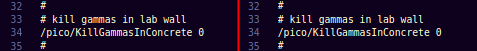
\includegraphics[scale = 1]{Images/gamma_wall.png}
		\caption{\label{tab:table-name}}
	\end{figure}

	\noindent The grdm commands allow you to use the full properties of the isotope. For the neutron source, I only cared about the neutron emission, which was modeled using calculations I had previously done. For gamma emission from the $^{207}$Bi source, I used the full isotope model. The key is the nucleusLimits variable which determines how far down the decay chain GEANT will track.
	
	\begin{figure}[!h]
		\centering
		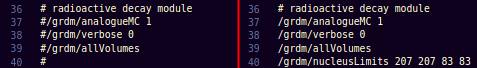
\includegraphics[scale = 1]{Images/grdm.png}
		\caption{\label{tab:table-name}}
	\end{figure}
	\pagebreak
	\noindent This block contains the meat of the macro file. It outlines all of the properties of the source, including its energy type (monoenergetic vs spectrum), energy(ies), angular distribution, position, size and shape, etc. Note, for grdm, I set the particle to be an ion. Here the energy refers to the movement of the ion itself, not the emitted particles. As a result, 0 energy means that the ion is sitting still in one spot.
	
	\begin{figure}[!h]
		\centering
		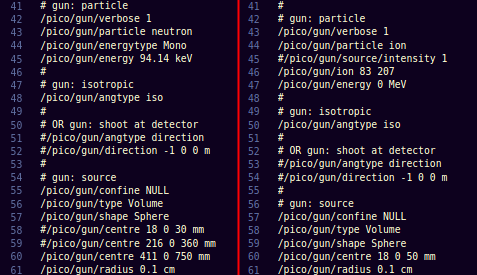
\includegraphics[scale = 1]{Images/properties.png}
		\caption{\label{tab:table-name}}
	\end{figure}

	\noindent Finally, this block details the names of the files that will be output. In particular, I used the neutron\_C3F8.out/gamma\_C3F8.out files for the analysis code in the next section. Also output is the neutron.root and gamma.root files, which are useful for using the ROOT program, although I did not use that much. Also in this block is the line for setting seeds, which was explained more in the section on my bash scripts. The final line is how many total emissions of the source GEANT will track, not the total hits on the target volume. So, 1000000 neutrons will be emitted from the source; however, you might only see a fraction of them recorded in the results. This number is very important in determining the real-time equivalent for a source, so keep track of it, as it is used in the analysis code in the next section.
	
	\begin{figure}[!h]
		\centering
		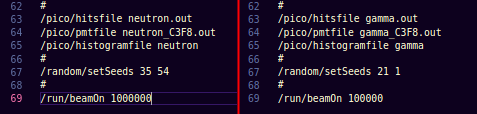
\includegraphics[scale = 1]{Images/output.png}
		\caption{\label{tab:table-name}}
	\end{figure}
	
	\section{Analysis Code}
	\par In this section, I'll discuss all of the code I wrote briefly in hopes that it is useful to you. I attempted to maintain good programming practices; however, as my thesis came to a close, I began to get a little sloppy, so hopefully nothing is too confusing to understand. All of these files are stored in the directory build/Analysis.
	\par The first file that I'll explain is create\_histograms.py. This file is the primary file to run for creating histograms and contains most of the setup. This file creates the plot as seen below in Figure 11 by making a histogram of the simulation results in the C3F8.out file, calculating the bubble rate per hour, and displaying the bubble nucleation threshold. The parameters are as follows: \\
	
	\begin{table}[!h]
		\begin{tabular}{ll}
			file\_list & \makecell[l]{- Full directory to either an exact C3F8.out file, or a folder containing many \\
				\indent .out files. All data will be plotted together as in Figure 11.}\\
			column\_id & - Column that you want to histogram. 6 is the deposited energy.\\
			tot\_events & \makecell[l]{- The total number of events the simulation ran for, as described at the end \\
				\indent of the previous section.}\\
			thresh & - Bubble nucleation threshold that you would like to see results for.\\
			rate & \makecell[l]{- The rate of emission of the source. For $^{207}$Bi, I had estimated a rate \\
				\indent of 0.3 neutrons/s.}\\
		\end{tabular}
	\end{table}
	
	\begin{figure}[!h]
		\centering
		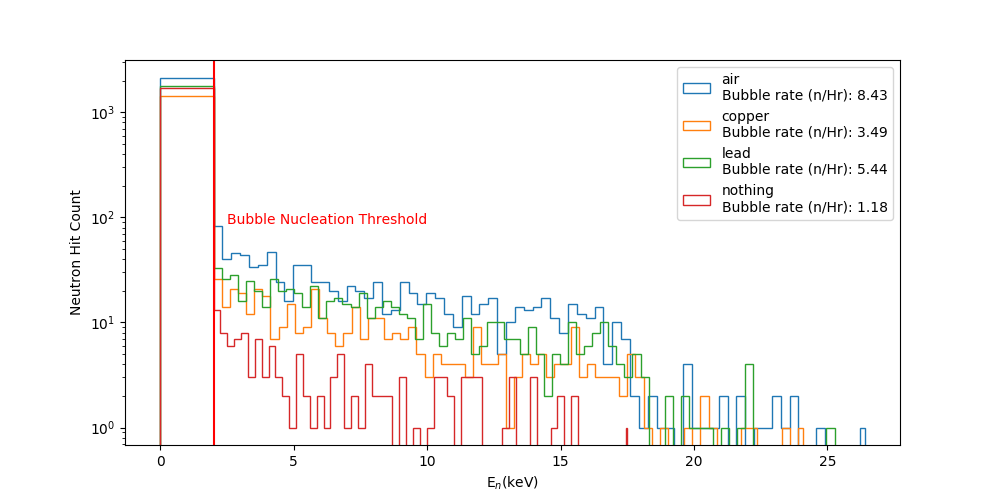
\includegraphics[scale = 0.65]{Images/particle_guide_log.png}
		\caption{\label{tab:table-name}}
	\end{figure}

	\begin{figure}[!t]
		\begin{minipage}{0.5\textwidth}
			\centering
			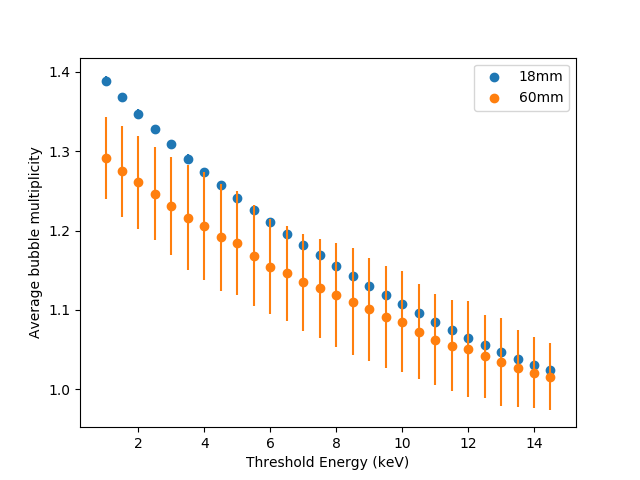
\includegraphics[width=1.1\linewidth]{Images/bubble_mult.png}
		\end{minipage}
		\begin{minipage}{0.5\textwidth}
			\centering
			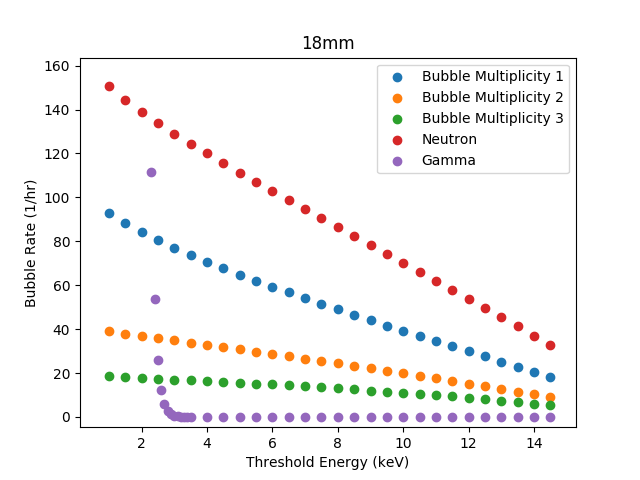
\includegraphics[width=1.1\linewidth]{Images/18mm_thresh.png}
		\end{minipage}
		\caption{\label{tab:table-name}}
	\end{figure}

	\par The next two files I'll discuss are secondary files split from create\_histograms.py to improve readability. These two are data\_operations.py and file\_operations.py. Since these are secondary files, you do not ever need to run them directly, and you should not have to make changes to them unless you discover a bug or need additional functionality. The file\_operations.py file performs the initial functions to read and load data from a file and column. The data\_operations.py performs all of the calculations such as bubble multiplicities, bubble rates, some statistics, and adds a histogram to the figure once calculations are finished.
	\par The bubble\_multiplicity.py file explores a wide range of bubble nucleation thresholds and calculates the average bubble multiplicity with error bars at each threshold. The results from one of my plots is shown above in Figure 12A. There are two different input combinations. The first is a single parameter with the full directory to a single C3F8.out file or a folder containing many C3F8.out files. The second combination is two parameters, each being the full directory to a file. This is how I created Figure 12A. There may be some bugs with the first case, because as I made changes, I sloppily did not check that previous functionality was preserved.
	\par The create\_threshold\_plot.py is used to similarly explore a range of bubble nucleation threshold energies, but this time, it calculates the expected bubble rate per hour for each threshold. I would guess that this file contains the sloppiest pieces of code, as I did not find a simple method to break down the rates by multiplicity, as seen in Figure 12B, without adding a method that reruns the entire loop again. As such, this code is fairly slow. In addition, this code was run on 100 simulations of 100000 events each. I do not know how it will function if you were to do a single simulation of 10000000 events. Something important to note is that this script uses data obtained from the PICO electron recoil paper to determine the gamma efficiency function to calculate bubble nucleations from gammas. The parameters are as follows:
	
	\begin{table}[!h]
		\begin{tabular}{ll}
			neutron\_path & \makecell[l]{- Full directory to the folder containing the neutron\_C3F8.out files.}\\
			gamma\_path & \makecell[l]{- Full directory to the folder containing the gamma\_C3F8.out files.}\\
			column\_id & - Column that you want to histogram. 6 is the deposited energy.\\
			tot\_events & \makecell[l]{- The total number of events the simulation ran for, as described at the end \\
				\indent of the previous section.}\\
			neutron\_ratee & \makecell[l]{- The rate of emission of the source. For $^{207}$Bi, I had estimated a rate \\
				\indent of 0.3 neutrons/s.}\\
			gamma\_ratee & \makecell[l]{- The rate of emission of the source. For $^{207}$Bi, I the source had a quoted \\
				\indent strength of 0.01 mCi or 370000 s$^{-1}$.}\\
		\end{tabular}
	\end{table}

	\begin{figure}[!t]
		\begin{minipage}{0.5\textwidth}
			\centering
			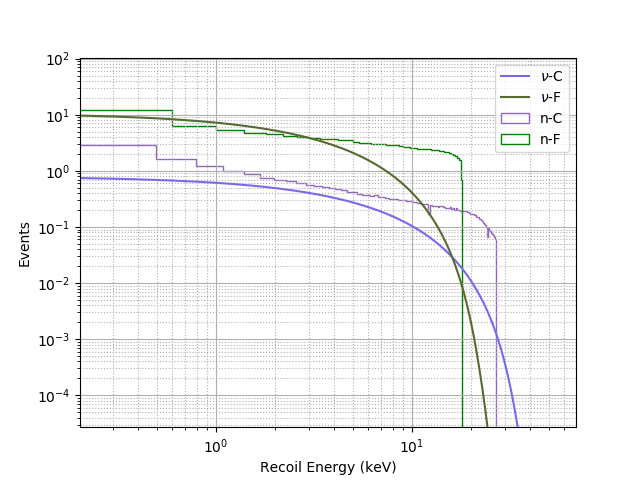
\includegraphics[width=1.1\linewidth]{Images/recoil_combined_normed.png}
		\end{minipage}
		\begin{minipage}{0.5\textwidth}
			\centering
			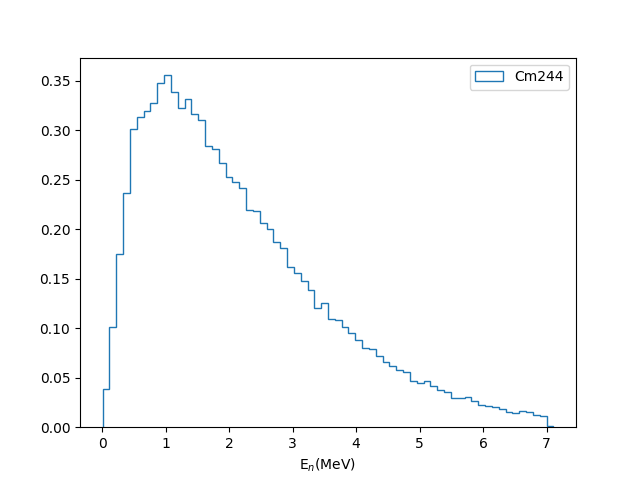
\includegraphics[width=1.1\linewidth]{Images/cm244_spectrum.png}
		\end{minipage}
		\caption{\label{tab:table-name}}
	\end{figure}

	\par The create\_split\_histograms.py file is an extension of the original histogram python script. This particular script was used to explored the possibility of the neutron spectrum resembling the $\nu$ spectrum. This script normalizes the neutron spectrum to match the $\nu$ spectrum at around 3 keV; however, the spectra did not match close enough as we had hoped. This script does not have much use outside of this scenario, so unless you are exploring a similar comparison of spectra, you will probably not need to use this script. Figure 13A shows what the output looked for the scenario I described above.
	\par The final two files work together to plot the spectrum of a non-monoenergetic source. This requires you to first pipe the output of the compile.sh script to some file. Then, the read\_output.sh script will scan that file for the energies and event numbers. Finally, the energy\_distribution.py file takes the output of the previous script and creates a histogram as seen in Figure 13B. This was useful to ensure that the spectrum of emitted particles matched what the actual source's spectrum would look like. These files won't be very useful for monoenergetic sources, and their only real use is if you suspect that there are issues with the emission spectra.
	
	\section{Conclusion}
	\par This manual was written fairly hastily, and as a result, it is not as clear and extensive as I would like it to be. Hopefully it has helped you in some way or another. If you make any changes to the simulation code, find errors or bugs anywhere, or add additional analysis code, feel free to update the manual as you see fit.

\end{document}